\section{Достоверность партонной модели при ПэВ-энергиях}
\label{sec:dis_reliability}

На рис.~(\ref{fig:xQ2_PDG}) показана область, исследованная в экспериментах на коллайдерах LHC, Tevatron и HERA, а также в экспериментах с неподвижной мишенью. 
В области малых значений $x \lesssim 10^{-6}$ экспериментальные данные практически отсутствуют. 
Между тем, с ростом энергии нейтрино вклад именно таких малых $x$ в полное сечение взаимодействия становится доминирующим. 
Выход за пределы экспериментально изученной области неизбежно требует экстраполяции партонных распределений, что влечёт дополнительную систематическую неопределённость в расчётах сечений.
\begin{figure}[!h]
\centering
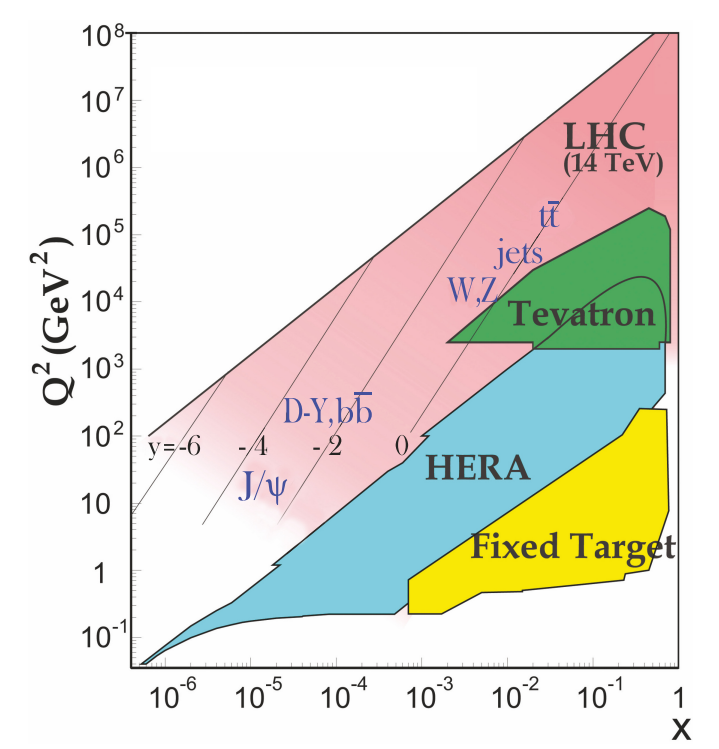
\includegraphics[width=0.8\linewidth]{images/NuProp/reald}
\caption{Кинематические области в $x$ и $Q^2$, исследованные в экспериментах с неподвижной мишенью и на коллайдерах. Рисунок из \cite{ParticleDataGroup:2024cfk}.}
\label{fig:xQ2_PDG}
\end{figure}

\subsection{Вклад экспериментально недоступной области}

Для иллюстрации на рис.~(\ref{fig:diff_xsec_100PeV}) показано дважды дифференциальное нормированное сечение
\[
\frac{1}{\sigma(E_\nu)}\frac{d^2\sigma(E_\nu,x,Q^2)}{dx\,dQ^2},
\]
представленное как функция переменных $x$ и $Q^2$ при энергии нейтрино $E_{\nu} = 100$~ПэВ. 
Здесь $\sigma(E_\nu)$ — полное сечение глубоконеупругого взаимодействия нейтрино с нуклоном при фиксированной энергии. 
На рисунке также заштрихована область, качественно отражающая диапазон экспериментальных измерений, показанный на рис.~(\ref{fig:xQ2_PDG}).

\begin{figure}[!h]
\centering
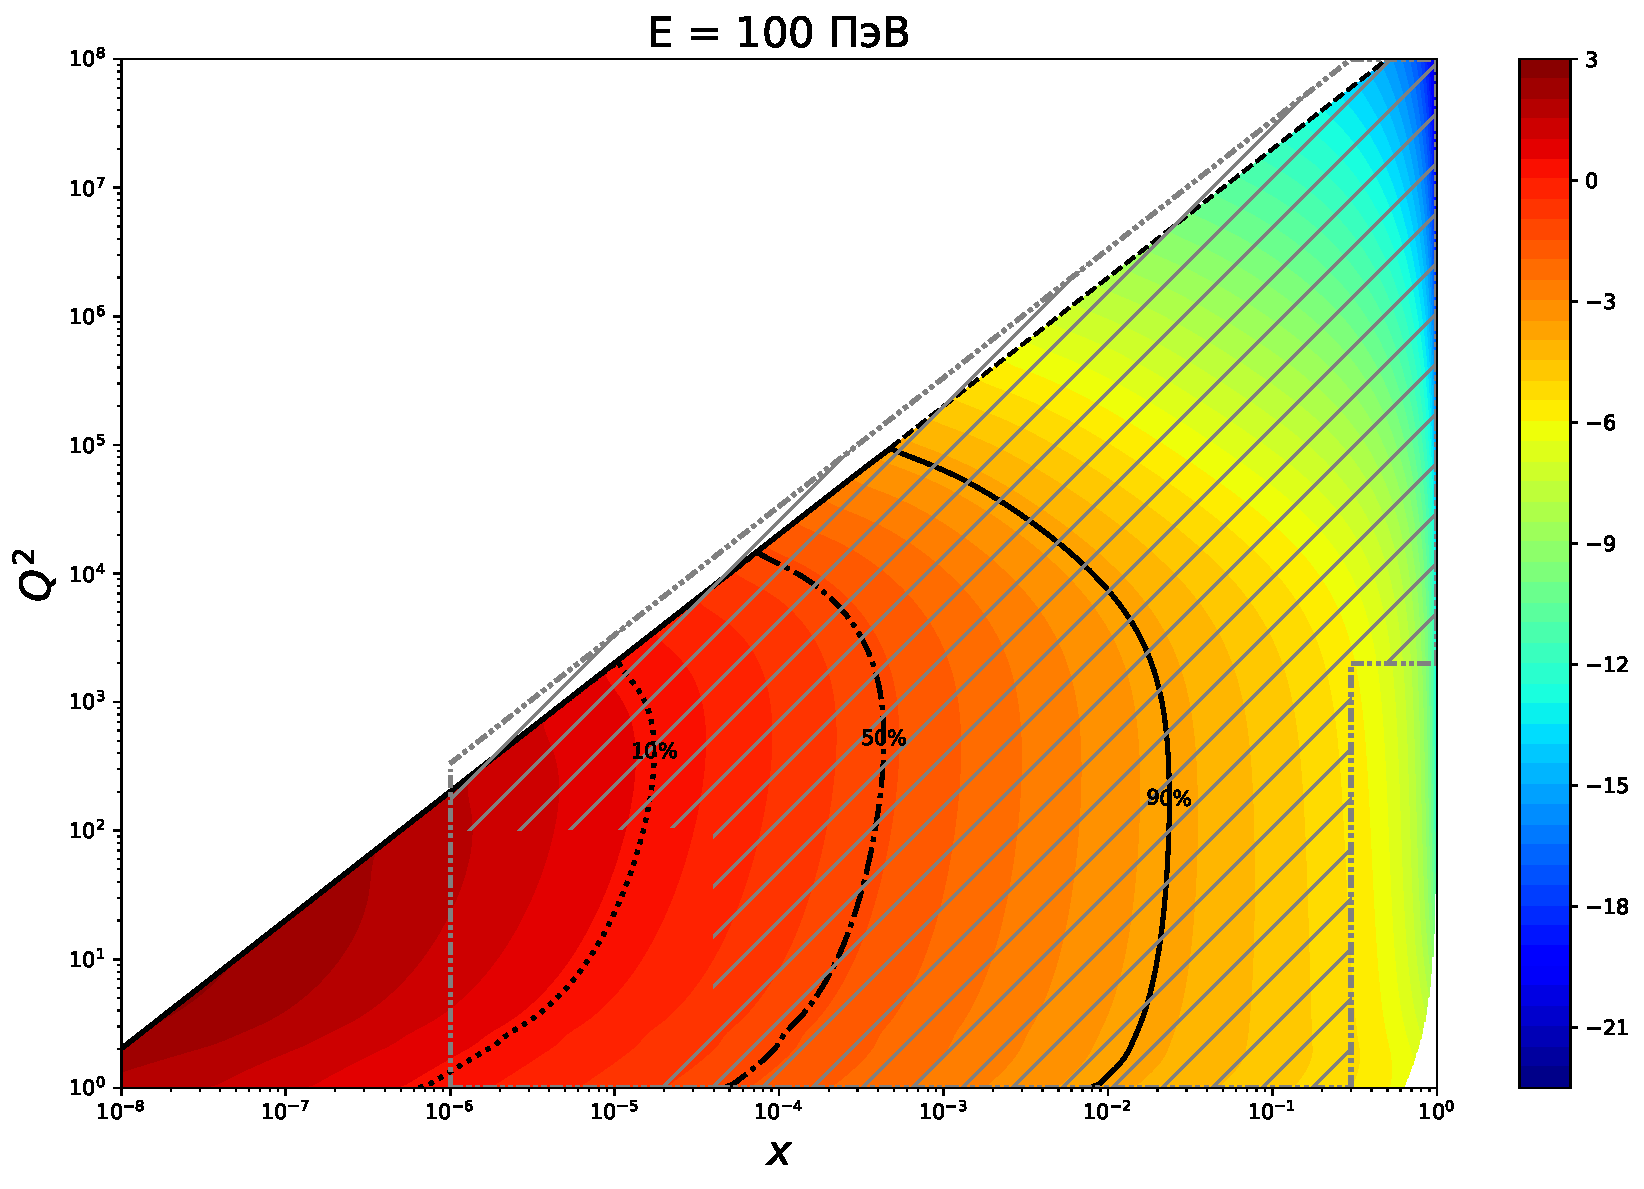
\includegraphics[width=0.6\linewidth]{images/NuProp/cdfxq2_cc_proton_CT18ZNNLO_14_100000000.pdf}
\caption{Дважды дифференциальное нормированное сечение 
$\frac{1}{\sigma(E_\nu)}\frac{d^2\sigma(E_\nu,x,Q^2)}{dx\,dQ^2}$ 
в зависимости от $x$ и $Q^2$ для энергии нейтрино $E_{\nu}=100$~ПэВ. 
Использованы партонные распределения CTEQ15~\cite{ncteq15}.}
\label{fig:diff_xsec_100PeV}
\end{figure}

В области $x \lesssim 10^{-6}$, где экспериментальные данные отсутствуют, величина 
$\frac{1}{\sigma(E_\nu)}\frac{d^2\sigma(E_\nu,x,Q^2)}{dx\,dQ^2}$ 
достигает максимальных значений. 
Пунктирные линии на рисунке указывают контуры, внутри которых вклад в полное сечение достигает $10\%$, $50\%$ и $90\%$ соответственно. 
Из анализа следует, что доля области $x \lesssim 10^{-6}$ в общем сечении составляет порядка $5\%$. 
В приложении~(\ref{sec:examples_extrapolated_region}) приведены два дополнительных примера аналогичных распределений для энергий нейтрино 1~ТэВ и 1~ПэВ.

Более простой способ оценки вклада неисследованной области заключается в том, чтобы пренебречь сложной зависимостью от двух переменных $x$ и $Q^2$ и рассматривать только наиболее значимую в данном контексте — переменную Бьёркена $x$. 
Определим отношение
\begin{equation}
\frac{1}{\sigma(E_\nu)}\int\limits_{x}^1 \frac{d\sigma(E_\nu,x')}{dx'}\,dx',
\label{eq:CDF_x}
\end{equation}
где
\[
\frac{d\sigma(E_\nu,x)}{dx} = \int\limits_0^{1} \frac{d^2\sigma(E_\nu,x,y)}{dx\,dy}\,dy.
\]

На рис.~(\ref{fig:CDF_x}) показана функция~(\ref{eq:CDF_x}) в зависимости от $x$ и $Q^2$ для трёх значений энергии нейтрино: $E_{\nu} = 1$~ТэВ, $1$~ПэВ и $100$~ПэВ.

\begin{figure}[!h]
\centering
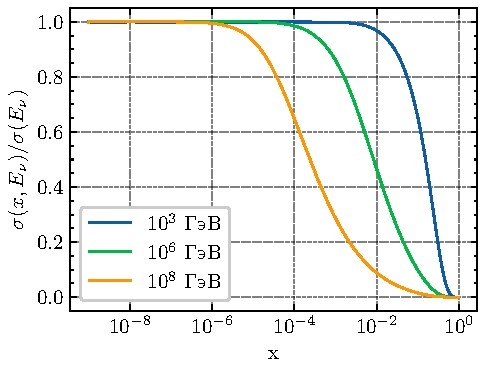
\includegraphics[width=0.8\linewidth]{images/NuProp/cdfxy_plot_CT18ZNNLO_14.pdf}
\caption{Функция 
$\int\limits_{x}^1 \frac{1}{\sigma(E_\nu)}\frac{d\sigma(E_\nu,x')}{dx'}\,dx'$ 
в зависимости от $x$ и $Q^2$ для трёх значений энергии нейтрино: 
$E_{\nu} = 1$~ТэВ, $1$~ПэВ и $100$~ПэВ. 
Использованы партонные распределения CTEQ15~\cite{ncteq15}.}
\label{fig:CDF_x}
\end{figure}


\subsection{Полное сечение и его вариация от параметризации}

Оценить вклад неисследованной области в величину полного сечения напрямую затруднительно. 
Более практичный подход состоит в сравнении результатов, получаемых при использовании различных параметризаций партонных распределений (PDF). 
Такой анализ позволяет оценить вариацию сечения, что включает экстраполяцию и разные теоретические схемы параметризаций PDF.

На рис.~(\ref{fig:xsec_total}) показана зависимость полного сечения взаимодействия мюонного нейтрино с нуклоном от энергии для нескольких современных наборов PDF. 
В  качестве базового набора PDF мы используем \texttt{CT10nlo}. 
Для оценки вариации полного сечения рассматриваются PDF от разных групп — \texttt{CT18ZNNLO}, \texttt{nCTEQ15} и \texttt{TUJU19\_nlo}. 
Такой выбор не претендует на полноту: он предназначен именно как срез «типичных» глобальных подгонок, отражающий вариацию теоретических оценок. 

Разброс значений полного сечения не превышает $\sim5\%$, что согласуется с оценками вклада неисследованной области, приведёнными выше.

\begin{figure}[!h]
\centering
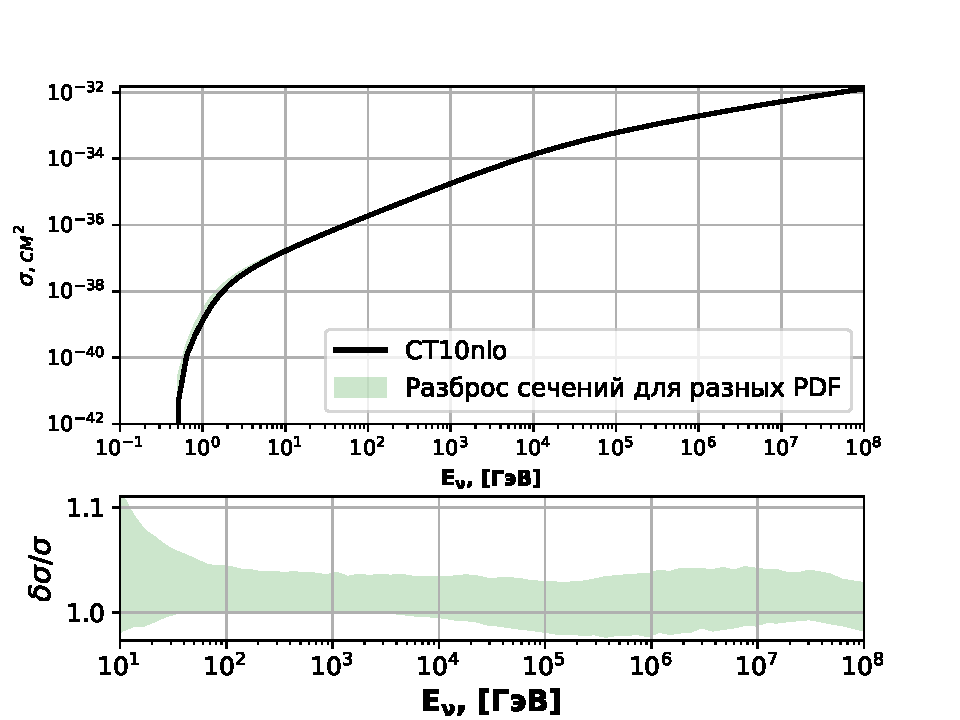
\includegraphics[width=\linewidth]{images/NuProp/xs_vs_enu.pdf}
\caption{Полные сечения взаимодействия мюонного нейтрино на нуклоне в зависимости от энергии $E_\nu$ для партонных распределений \texttt{CT10nlo}. 
Полоса отражает вариацию полного сечения при использовании других наборов PDF (\texttt{CT18ZNNLO}, \texttt{nCTEQ15}, \texttt{TUJU19\_nlo}).} 
\label{fig:xsec_total}
\end{figure}
